\documentclass[11pt]{article}

\usepackage{amsmath}
\usepackage{amssymb}

\usepackage{graphicx}

\usepackage{ytableau}

\title{Matchings, \\ Math 4707, Spring 2021}
\date{}

\begin{document}

\maketitle

\thispagestyle{empty}

\begin{enumerate}
\item Let $G$ be the following bipartite graph on 12 vertices:
\[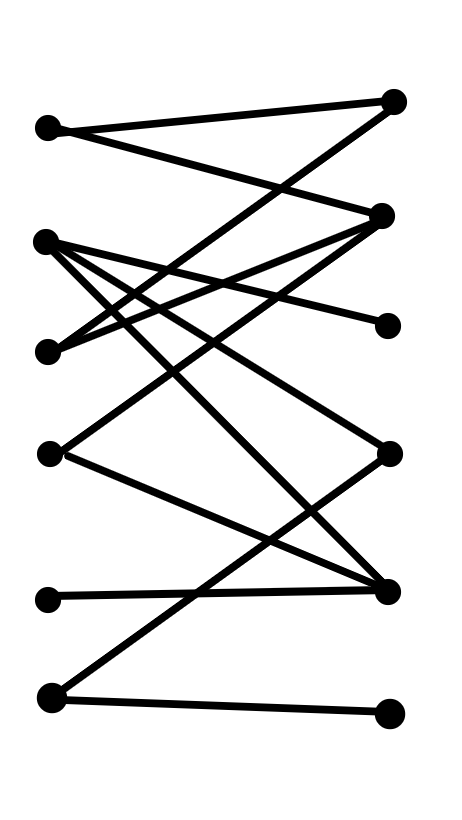
\includegraphics[width=1in]{matching.png}\]
Find a matching of $G$ with the maximum possible number of edges. How do you \emph{know} that this is the maximum?
\item Let $G$ be a simple bipartite graph with bipartition $(X,Y)$. Suppose that $n=\#X=\#Y$ (so the total number of vertices of $G$ is $2n$).
\begin{enumerate}
\item If $G$ has a perfect matching, must it be connected?
\item What is the fewest number of edges $G$ could have if it has a perfect matching.
\item Show that $G$ can have $n^2-n$ edges but still fail to have a perfect matching.
\item Show that if $G$ has at least $n^2-n+1$ edges, then it must have a perfect matching. \\
{\bf Hint}: suppose there is a subset $A\subseteq X$ with $a = \#A > \#N_G(A)$, where $N_G(A)$ denotes the neighborhood of $A$ in $G$. Write an expression (in terms of $a$ and $n$) for the maximum possible number of edges $G$ could have in that case. Show that your expression cannot be greater than or equal to $n^2-n+1$.
\end{enumerate}
\end{enumerate}

\end{document}
